\subsection{Stage 5a --- Auxiliary Composition Surrogate}
\label{sec:comp_nn}

This is the dashed side-branch in Figure~\ref{fig:pipeline}. It is separate
from the potential-fitting flow: it reads the Stage~2 MD output directly and
never feeds back into it. Its job is to be a fast check on the consistency of
the LAMMPS dataset. If a composition-only network cannot recover even a rough
$(E,\nu)$ trend from the data, the MD output itself is suspect. As a useful
side effect, the trained network doubles as a quick predictor for new
compositions.

Each input vector has 12 entries, one mass fraction per element in
$\{$Al, Co, Cr, Cu, Fe, Mg, Mn, Mo, Ni, Si, Ti, Zn$\}$. The network is a
fully-connected $12\to32\to20\to2$ MLP with ReLU activations, trained under a
70/30 train/validation split with Adam. To get a usable uncertainty estimate,
five copies are trained from different random seeds and combined as a deep
ensemble \citep{lakshminarayanan2017}; the spread across the ensemble flags
inputs the network is unsure about.

\paragraph{Targets and Huber loss.}
The two outputs are $C_{11}$ and $C_{12}$, and $(E,\nu)$ are recovered from
Eq.~\eqref{eq:elastic} afterwards, for the conditioning reason given in
Section~\ref{sec:stage2}. Records with $\nu\geq0.48$ are dropped to remove
compositions that sit on the mechanical-stability bound and destabilise the
fit. The loss is Huber ($\delta=1$ in scaled units) rather than MSE, which
caps the gradient pull of outliers, mostly the Mg- and Zn-rich runs that
occasionally return extreme moduli.

\paragraph{Performance.}
On the held-out 30\,\% split the network reaches $R^2 = 0.77$ on $E$ and
$R^2 = 0.52$ on $\nu$, with the full per-target breakdown in
Table~\ref{tab:nn_aux}. The lower $\nu$ score is the expected cost of taking a
ratio of two learned constants near the point where their difference is small.
As a concrete check, feeding the Al~7075 composition through the ensemble
returns $\hat E = 75.5$\,GPa and $\hat\nu = 0.334$, against the published
$71$ to $72$\,GPa and $\nu\approx0.33$, an error of about $5\,\%$. The parity
plots in Figure~\ref{fig:aux_parity} show this both on the raw $(C_{11},C_{12})$
targets and on the derived $(E,\nu)$, and the training history is in
Figure~\ref{fig:aux_history}.

% AUTO-GENERATED by src/ML/nn_alloy.py -- do not edit
\begin{table}[htbp]
\centering
\caption{Performance of the composition surrogate (N=7839; train=5487, val=2352).}
\label{tab:nn_aux}
\begin{tabular}{lrrrrrrl}
\hline
 Split / Target            &    MAE &   RMSE &    Std &   Bias &   $R^2$ &   $r$ & MAPE       \\
\hline
 Train, $C_{11}$ (GPa)     & 14.515 & 23.782 & 23.136 & -5.512 &   0.967 & 0.985 & 7.140\,\%  \\
 Train, $C_{12}$ (GPa)     & 10.092 & 18.811 & 18.643 & -2.522 &   0.963 & 0.982 & 14.511\,\% \\
 Train, $E$ (GPa, derived) & 18.037 & 28.176 & 27.999 & -3.174 &   0.860 & 0.929 & 14.492\,\% \\
 Train, $\nu$ (derived)    &  0.025 &  0.036 &  0.036 &  0.001 &   0.693 & 0.833 & 10.318\,\% \\
 Val., $C_{11}$ (GPa)      & 19.745 & 64.147 & 63.928 & -5.456 &   0.646 & 0.822 & 8.563\,\%  \\
 Val., $C_{12}$ (GPa)      & 14.318 & 57.325 & 57.272 & -2.729 &   0.364 & 0.683 & 14.368\,\% \\
 Val., $E$ (GPa, derived)  & 20.436 & 34.975 & 34.864 & -2.881 &   0.770 & 0.878 & 16.272\,\% \\
 Val., $\nu$ (derived)     &  0.027 &  0.043 &  0.043 &  0.001 &   0.518 & 0.731 & 10.604\,\% \\
\hline
\end{tabular}
\end{table}


\begin{figure}[h]
	\centering
	\begin{minipage}[t]{0.48\textwidth}
		\centering
		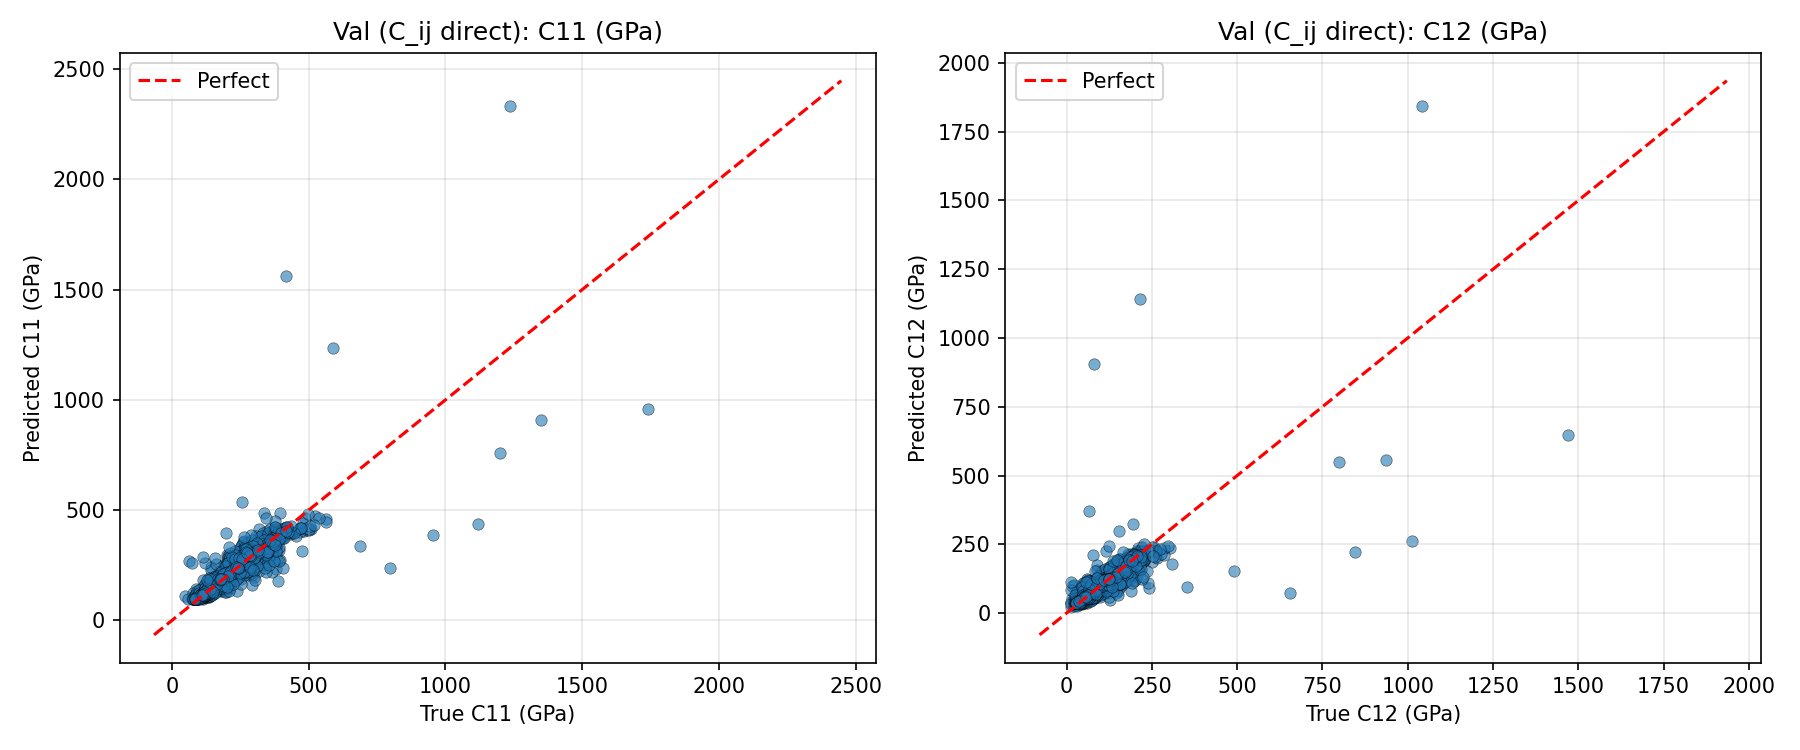
\includegraphics[width=\textwidth]{figures/parity_validation_cij.png}
		\caption{Held-out parity on the raw targets $C_{11}$ and $C_{12}$,
		the quantities the network actually regresses.}
		\label{fig:aux_parity}
	\end{minipage}
	\hfill
	\begin{minipage}[t]{0.48\textwidth}
		\centering
		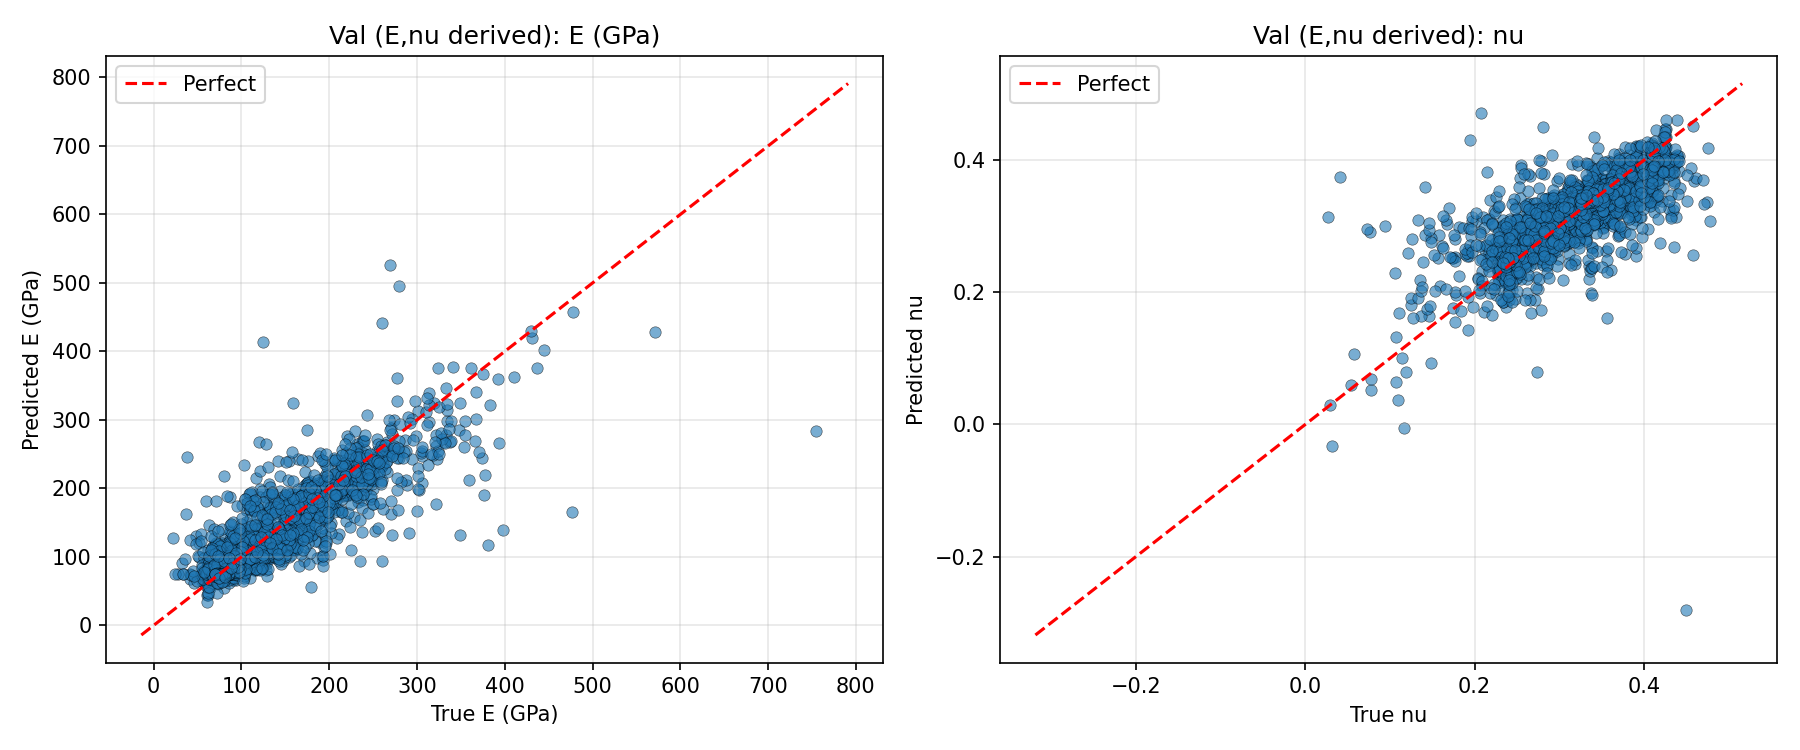
\includegraphics[width=\textwidth]{figures/parity_validation.png}
		\caption{Held-out parity on the derived $(E,\nu)$, recovered from the
		predicted constants through Eq.~\eqref{eq:elastic}.}
		\label{fig:aux_parity_val}
	\end{minipage}
\end{figure}

\begin{figure}[h]
	\centering
	\begin{minipage}[t]{0.48\textwidth}
		\centering
		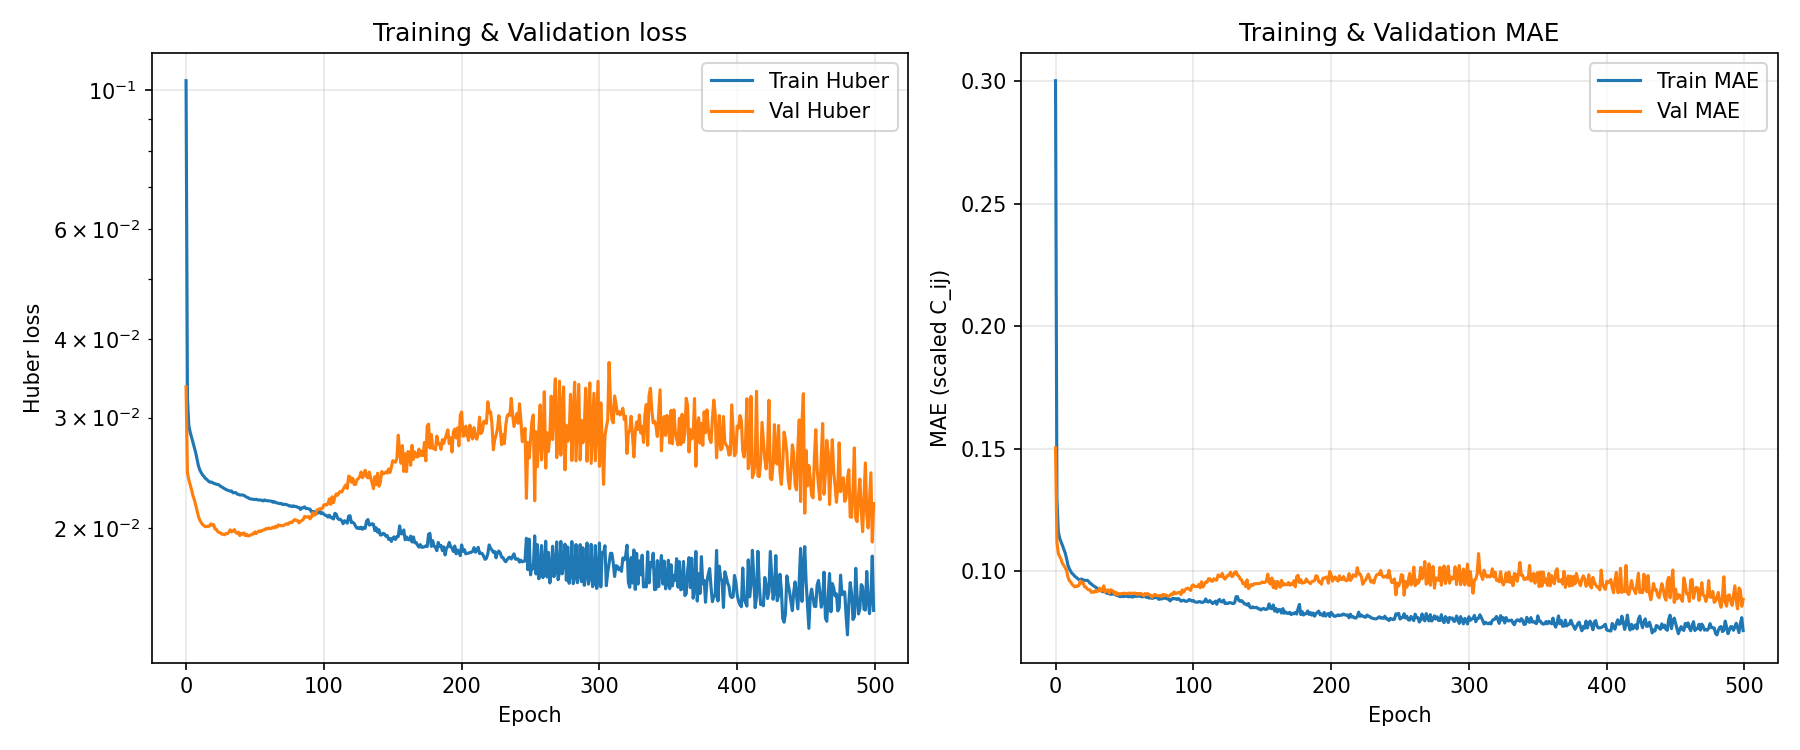
\includegraphics[width=\textwidth]{figures/training_history.png}
		\caption{Training history: Huber loss and MAE on the scaled targets.}
		\label{fig:aux_history}
	\end{minipage}
	\hfill
	\begin{minipage}[t]{0.48\textwidth}
		\centering
		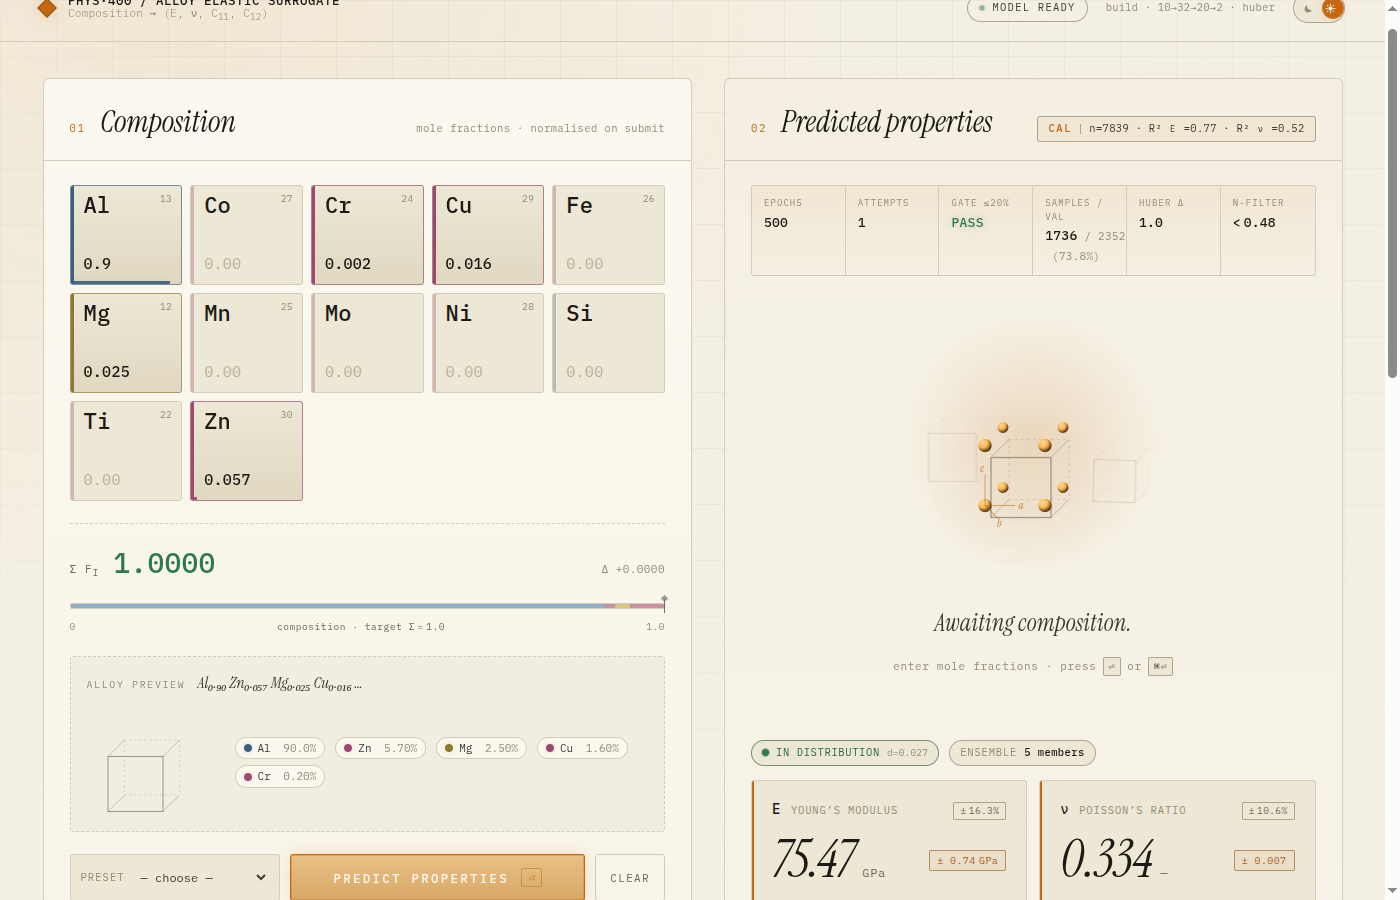
\includegraphics[width=\textwidth]{figures/ml_app.png}
		\caption{The surrogate packaged as a portable predictor. A composition
		is entered on the simplex and the ensemble returns $(E,\nu)$ with a
		$k$-nearest-neighbour distance flag for out-of-distribution inputs.}
		\label{fig:aux_app}
	\end{minipage}
\end{figure}

The surrogate is shipped as a portable application image with a small Flask
front end, so a composition can be entered and scored without touching the
training code. A $k$-nearest-neighbour distance in composition space is
reported alongside each prediction; when an input sits far from the training
cloud, the flag warns that the answer is an extrapolation.
